% id: 0566
% book: 쎈 중3-2 수학 · 05 원주각의 활용
% section: 유형 10 접선과 현이 이루는 각의 활용 (2)
% figure: tikz:fig-0566
% answer: ①
% answer_source: 답지
% variant_level: 0 (원본 전사)
% 이 파일은 build.mjs 가 items.json 에서 만든다. 고칠 때는 items.json 을 고친다.
\smash{\raisebox{1.5mm}{\dmkichul{쎈 중3-2 수학 0566번 · 102쪽}}}
\noindent\begin{minipage}[t]{0.58\linewidth}\vspace{0pt}\raggedright 오른쪽 그림에서 점~$\pt{P}$는 원~$\pt{O}$의 지름~$\pt{AB}$의 연장선과 원 위의 점~$\pt{T}$에서의 접선의 교점이다. $\angle\pt{BCT}=65^\circ$일 때, $\angle x$의 크기는?\end{minipage}\hfill\begin{minipage}[t]{0.4\linewidth}\vspace{0pt}\centering \resizebox{\ifdim\width>\linewidth\linewidth\else\width\fi}{!}{% 0566(본책 102쪽) — 원 O, 지름 AB 연장선과 접점 T 의 접선의 교점 P, ∠BCT=65°, ∠x(∠APT). 스캔 삽화를 TikZ 로 다시 그림. 답은 적지 않는다.
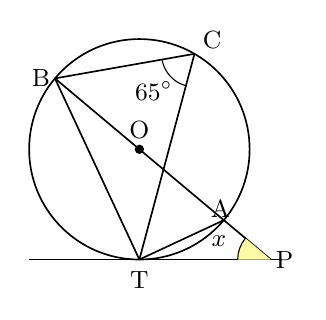
\begin{tikzpicture}[scale=1.4, line width=0.6pt]
  \draw (0.000,0.000) circle (1.000);
  \draw (-1.000,-1.000) -- (1.292,-1.000);
  \draw (-0.766,0.643) -- (1.192,-1.000);
  \draw (-0.766,0.643) -- (0.500,0.866);
  \draw (0.500,0.866) -- (-0.000,-1.000);
  \draw (-0.766,0.643) -- (-0.000,-1.000);
  \draw (0.766,-0.643) -- (-0.000,-1.000);
  \fill (0.000,0.000) circle (1.2pt);
  \draw[line width=0.4pt] (0.205,0.814) arc[start angle=-170.000, end angle=-105.000, radius=0.300];
  \node[font=\small, inner sep=1pt] at (0.131,0.528) {$65^\circ$};
  \fill[yellow!35] (1.192,-1.000) -- ++(140.000:0.300) arc[start angle=140.000, end angle=180.000, radius=0.300] -- cycle;
  \draw[line width=0.4pt] (0.962,-0.807) arc[start angle=140.000, end angle=180.000, radius=0.300];
  \node[font=\small, inner sep=1pt] at (0.722,-0.829) {$x$};
  \node[font=\small, anchor=south, inner sep=1.5pt] at (0.000,0.050) {O};
  \node[font=\small, anchor=east, inner sep=1.5pt] at (-0.766,0.643) {B};
  \node[font=\small, anchor=south west, inner sep=1.5pt] at (0.530,0.866) {C};
  \node[font=\small, anchor=south, inner sep=1.5pt] at (0.736,-0.663) {A};
  \node[font=\small, anchor=west, inner sep=1.5pt] at (1.192,-1.000) {P};
  \node[font=\small, anchor=north, inner sep=1.5pt] at (-0.000,-1.060) {T};
\end{tikzpicture}
}\end{minipage}\par
\begin{choices32}{$40^\circ$}{$43^\circ$}{$45^\circ$}{$48^\circ$}{$50^\circ$}\end{choices32}
